
\documentclass[a4paper,12pt]{article} % тип документа


% Русский язык
\usepackage[T2A]{fontenc} % кодировка
\usepackage[utf8]{inputenc} % кодировка исходного текста
\usepackage[russian,english]{babel} % локализация и переносы
\usepackage{graphicx}
\graphicspath{{pictures/}}
\DeclareGraphicsExtensions{.pdf,.png,.jpg}

\newenvironment{comment}{}{}


% Математика
\usepackage{amsmath,amsfonts,amssymb,amsthm,mathtools}


\usepackage{wasysym}

\begin{document}


\begin{center}
\includegraphics{10}
\end{center}
\begin{center}
\includegraphics{1}
\end{center}


\begin{center}
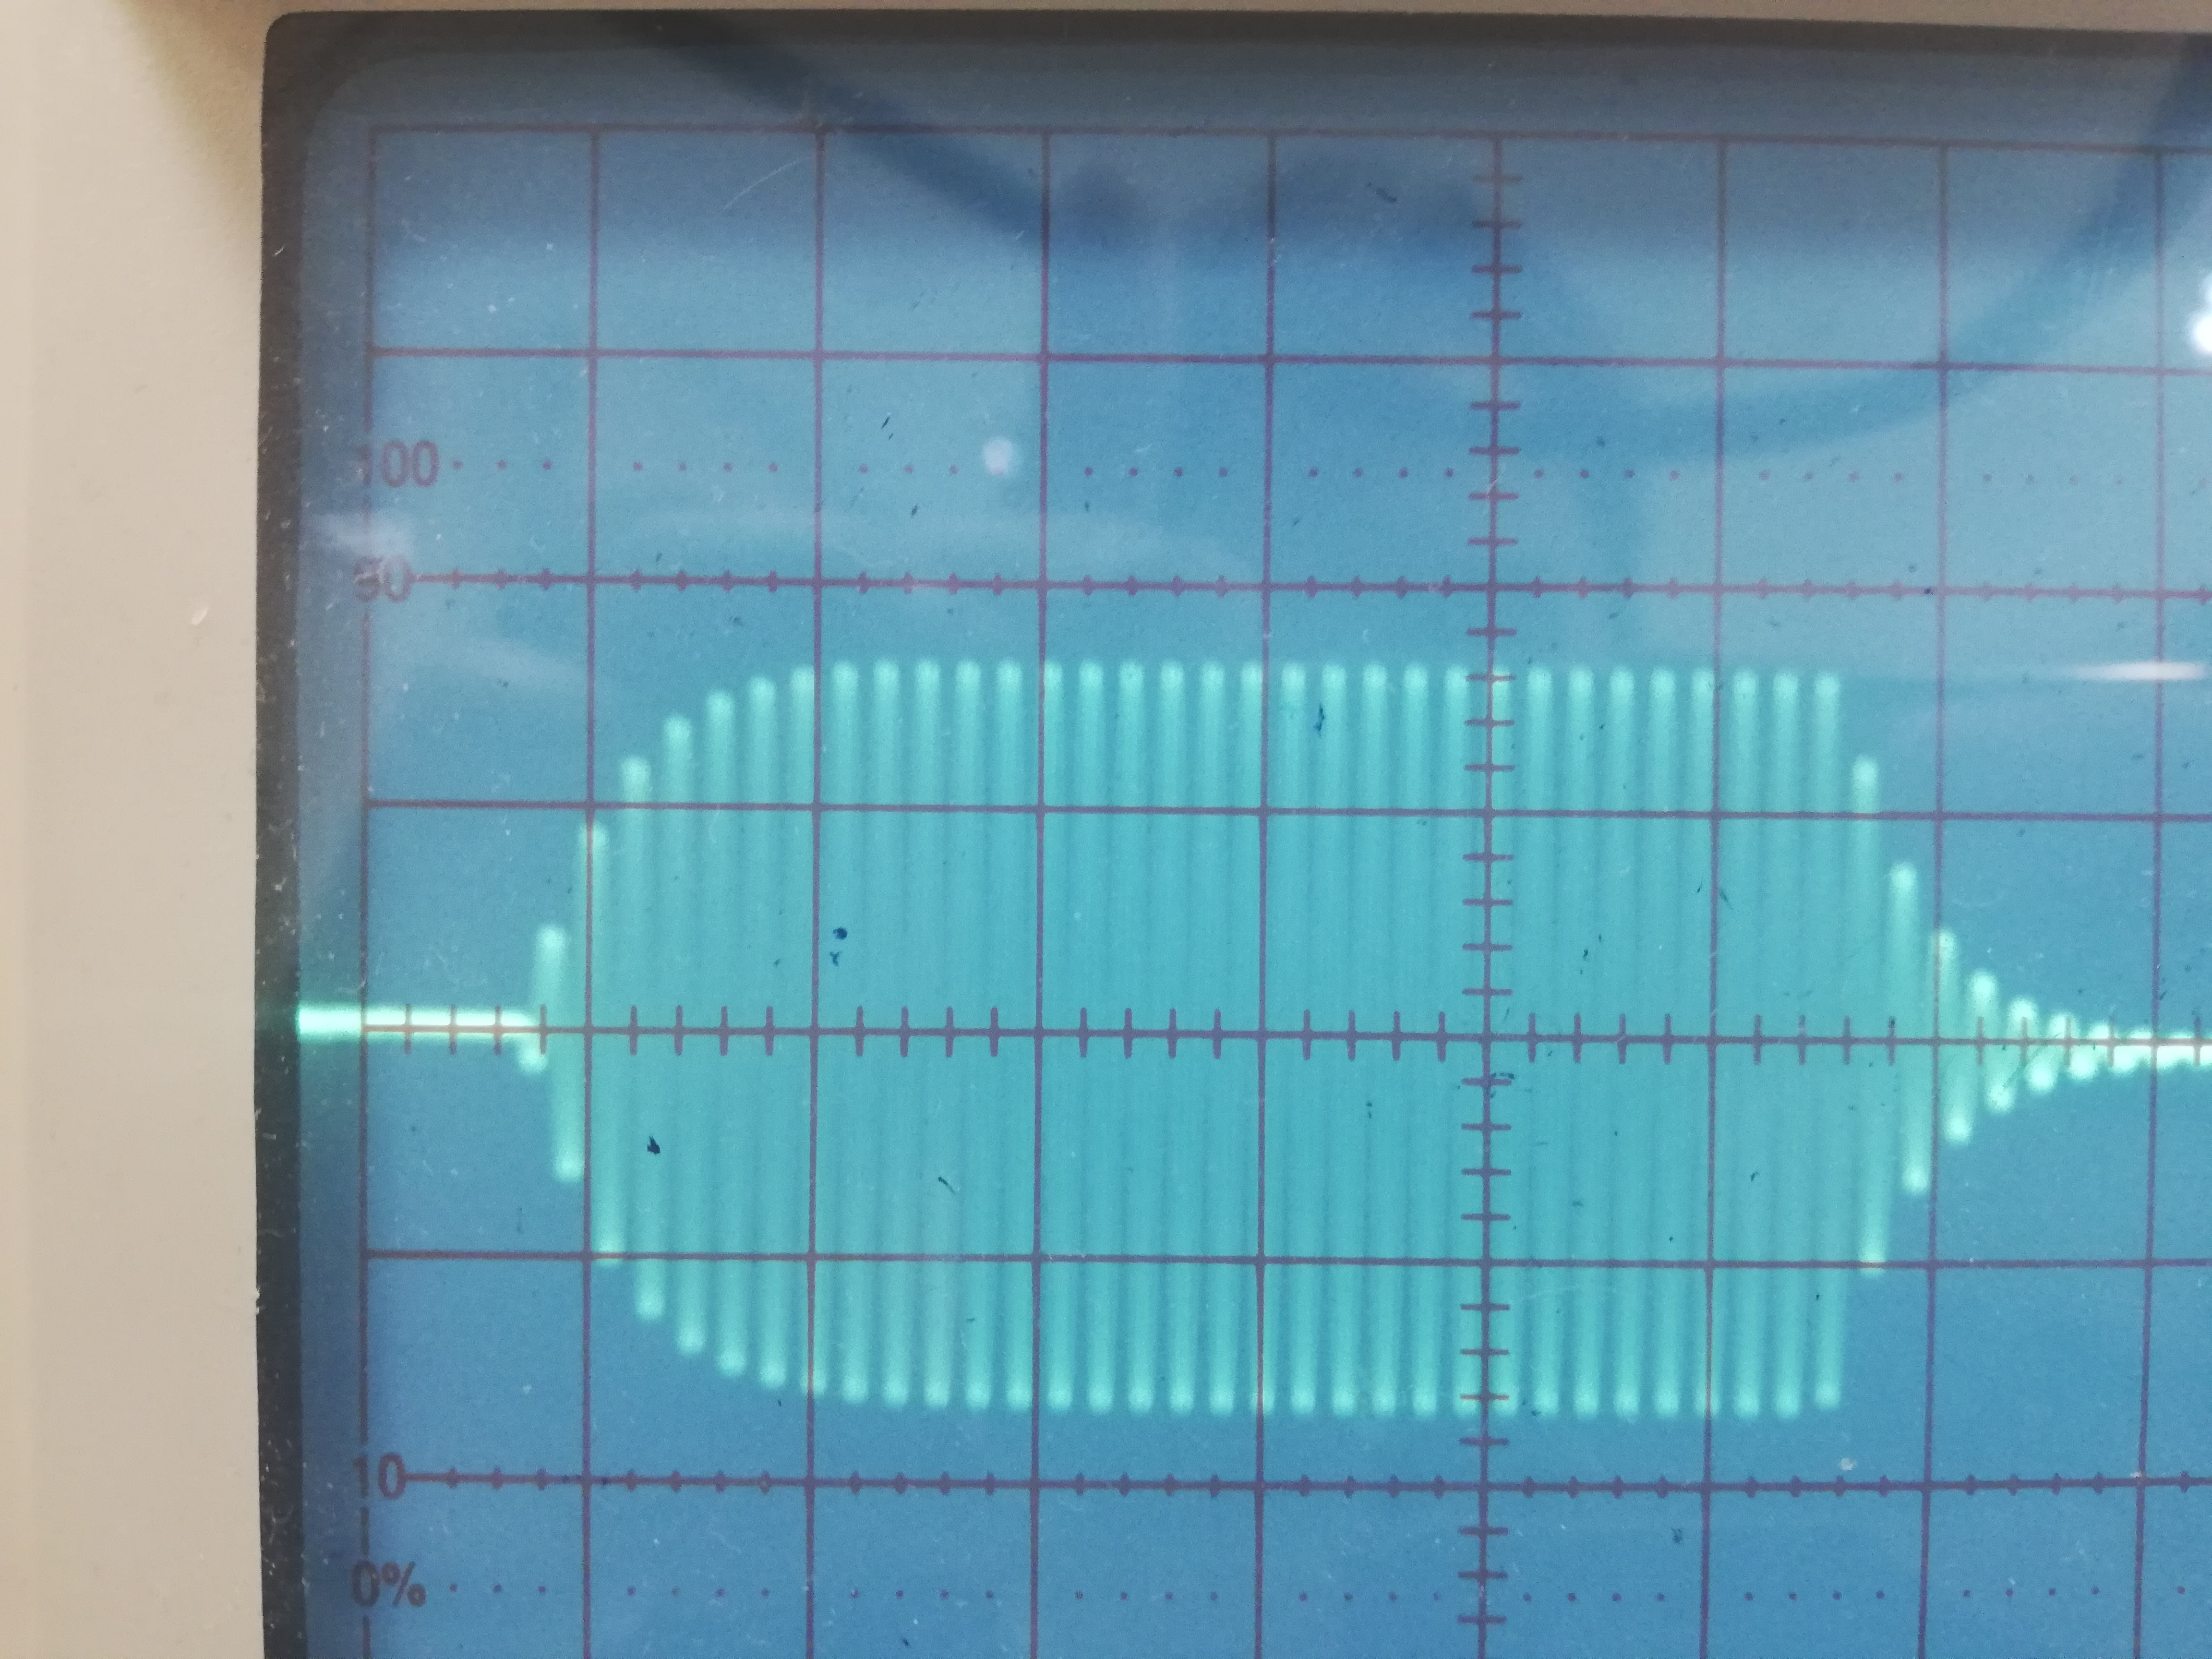
\includegraphics{2}
\end{center}
\begin{center}
\includegraphics{4}
\end{center}
\begin{center}
\includegraphics{5}
\end{center}
\begin{center}
\includegraphics{6}
\end{center}
\begin{center}
\includegraphics{7}
\end{center}

\begin{center}
\includegraphics{8}
\end{center}
\begin{center}
\includegraphics{9}
\end{center}

\begin{center}
\includegraphics{11}
\end{center}

\begin{center}
\includegraphics{12}
\end{center}
\begin{center}
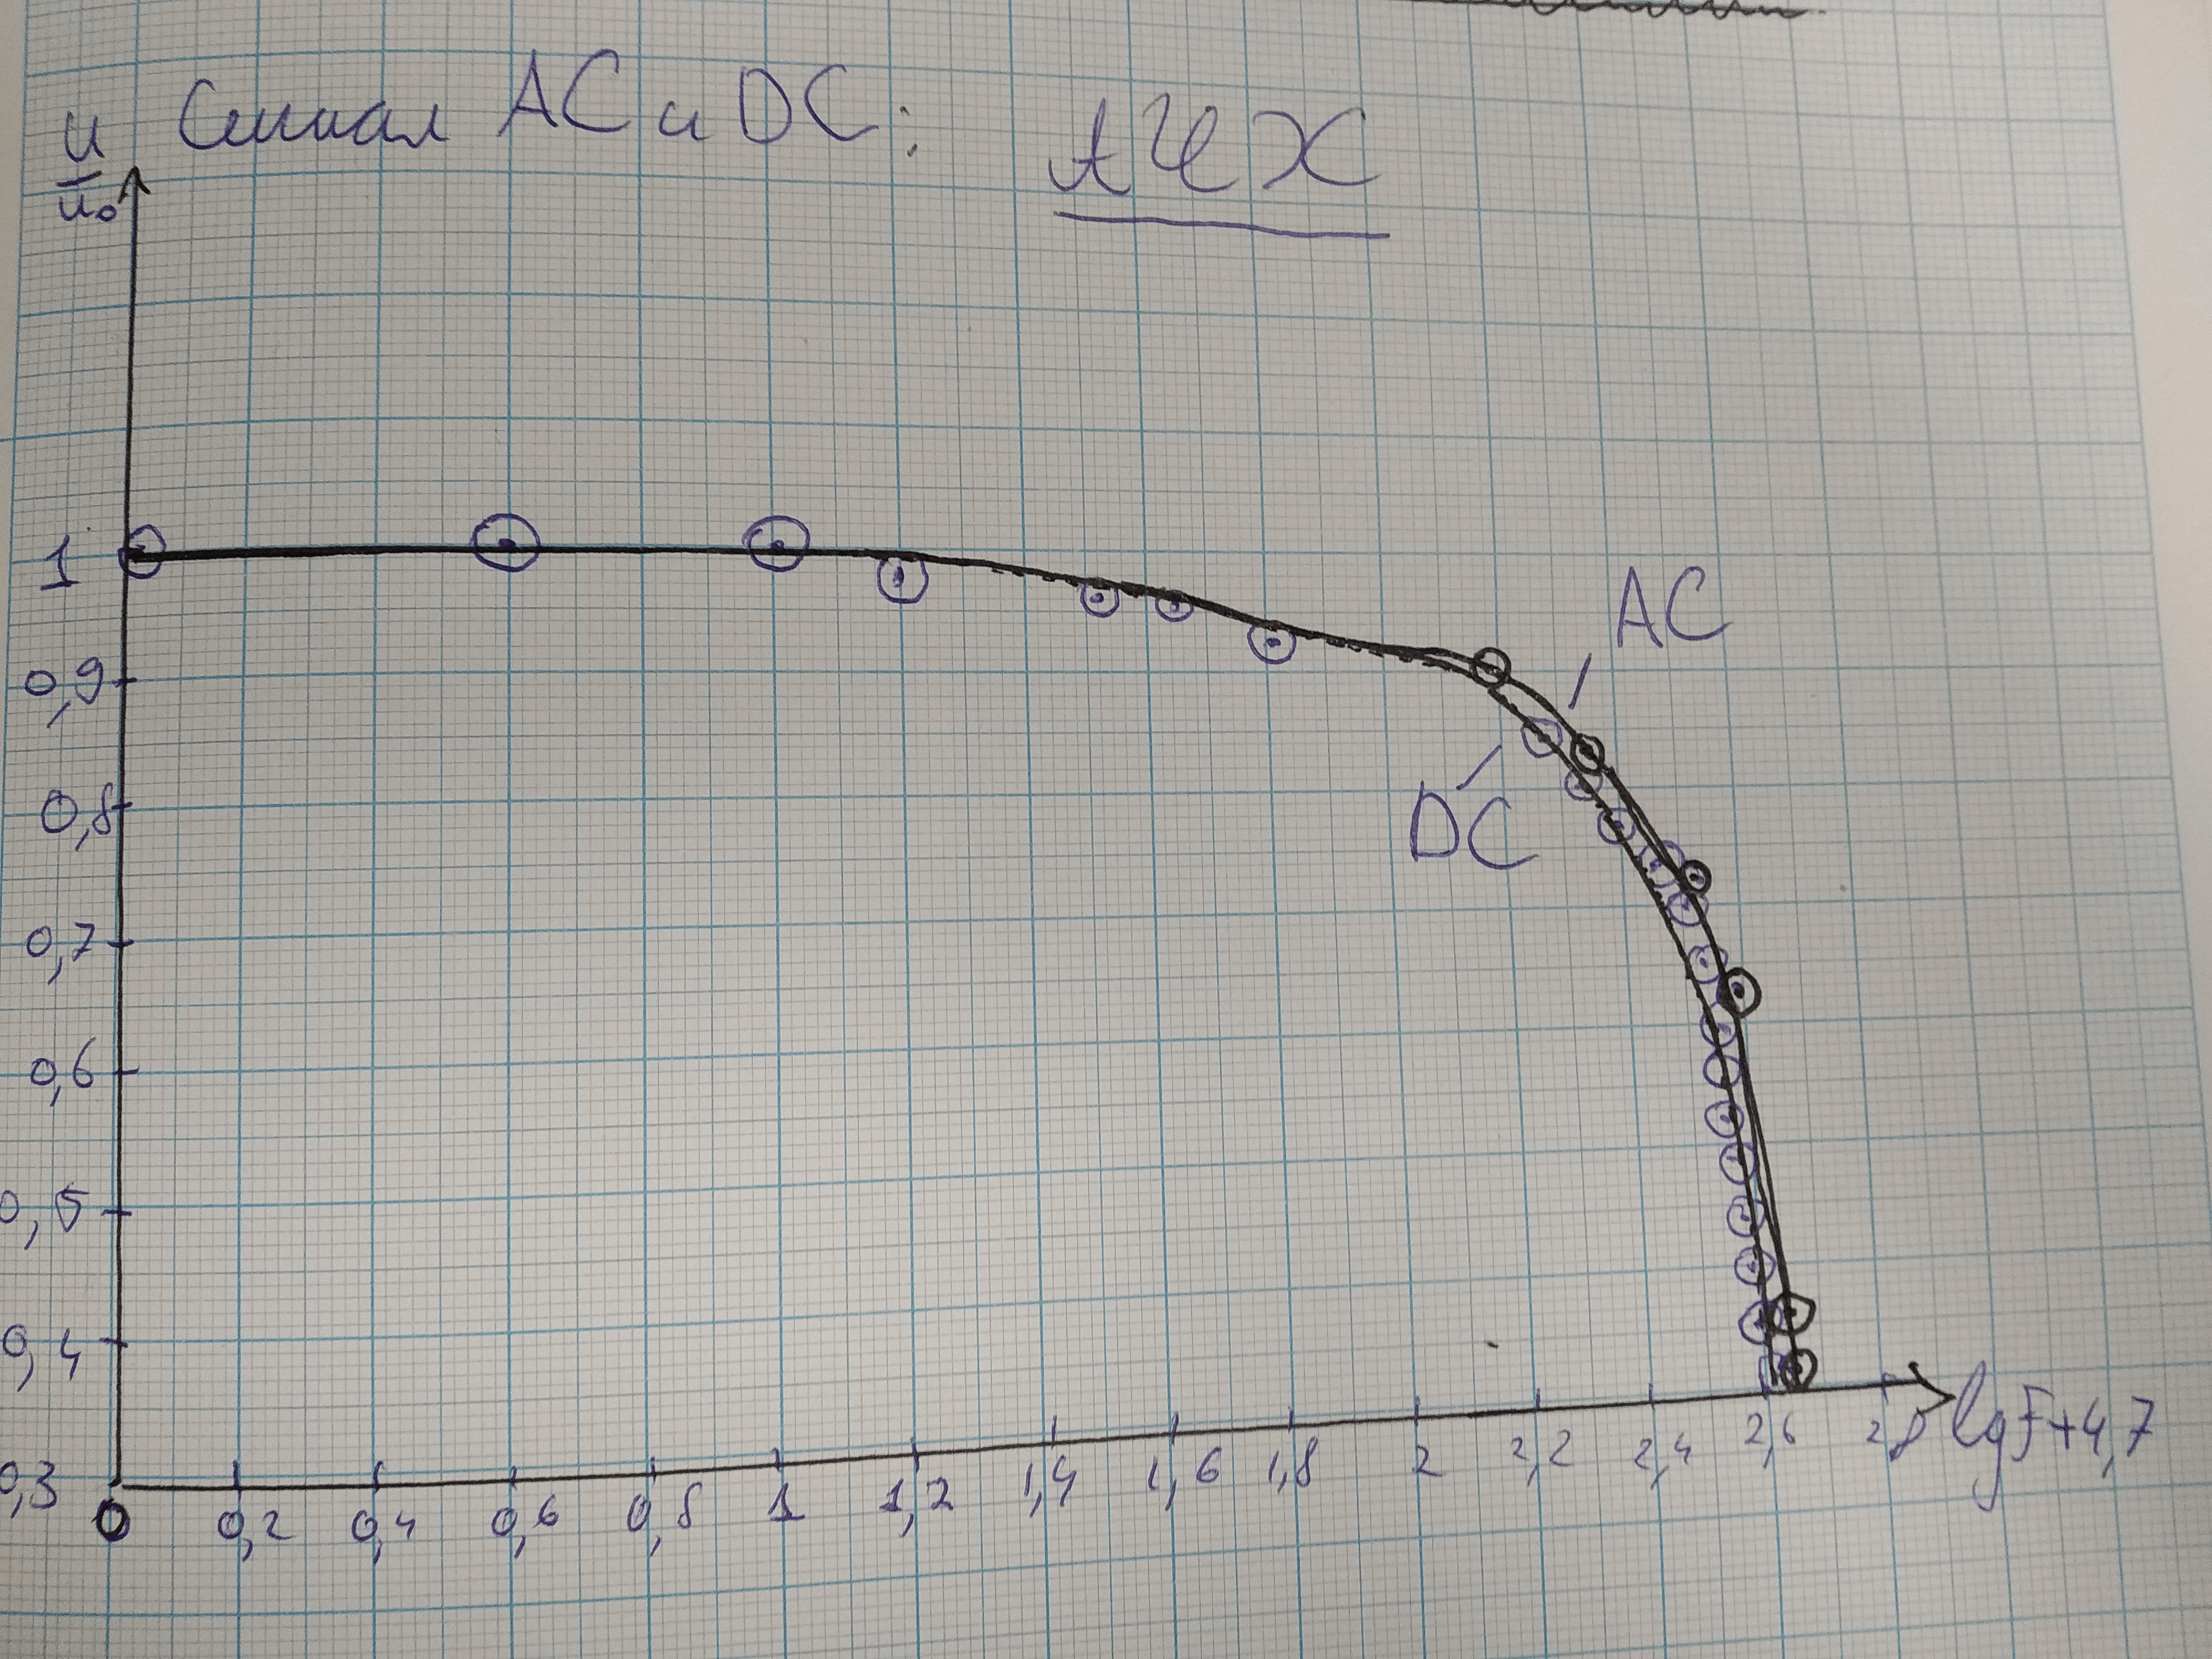
\includegraphics[width=120mm]{13}
\end{center}

\begin{center}
\includegraphics{14}
\end{center}

\begin{center}
\includegraphics{15}
\end{center}

\begin{center}
\includegraphics{16}
\end{center}

\begin{center}
\includegraphics{17}
\end{center}

\begin{center}
\includegraphics{18}
\end{center}

\begin{center}
\includegraphics{19}
\end{center}

\begin{center}
\includegraphics{20}
\end{center}

\begin{center}
\includegraphics{21}
\end{center}

\begin{center}
\includegraphics{22}
\end{center}


\begin{center}
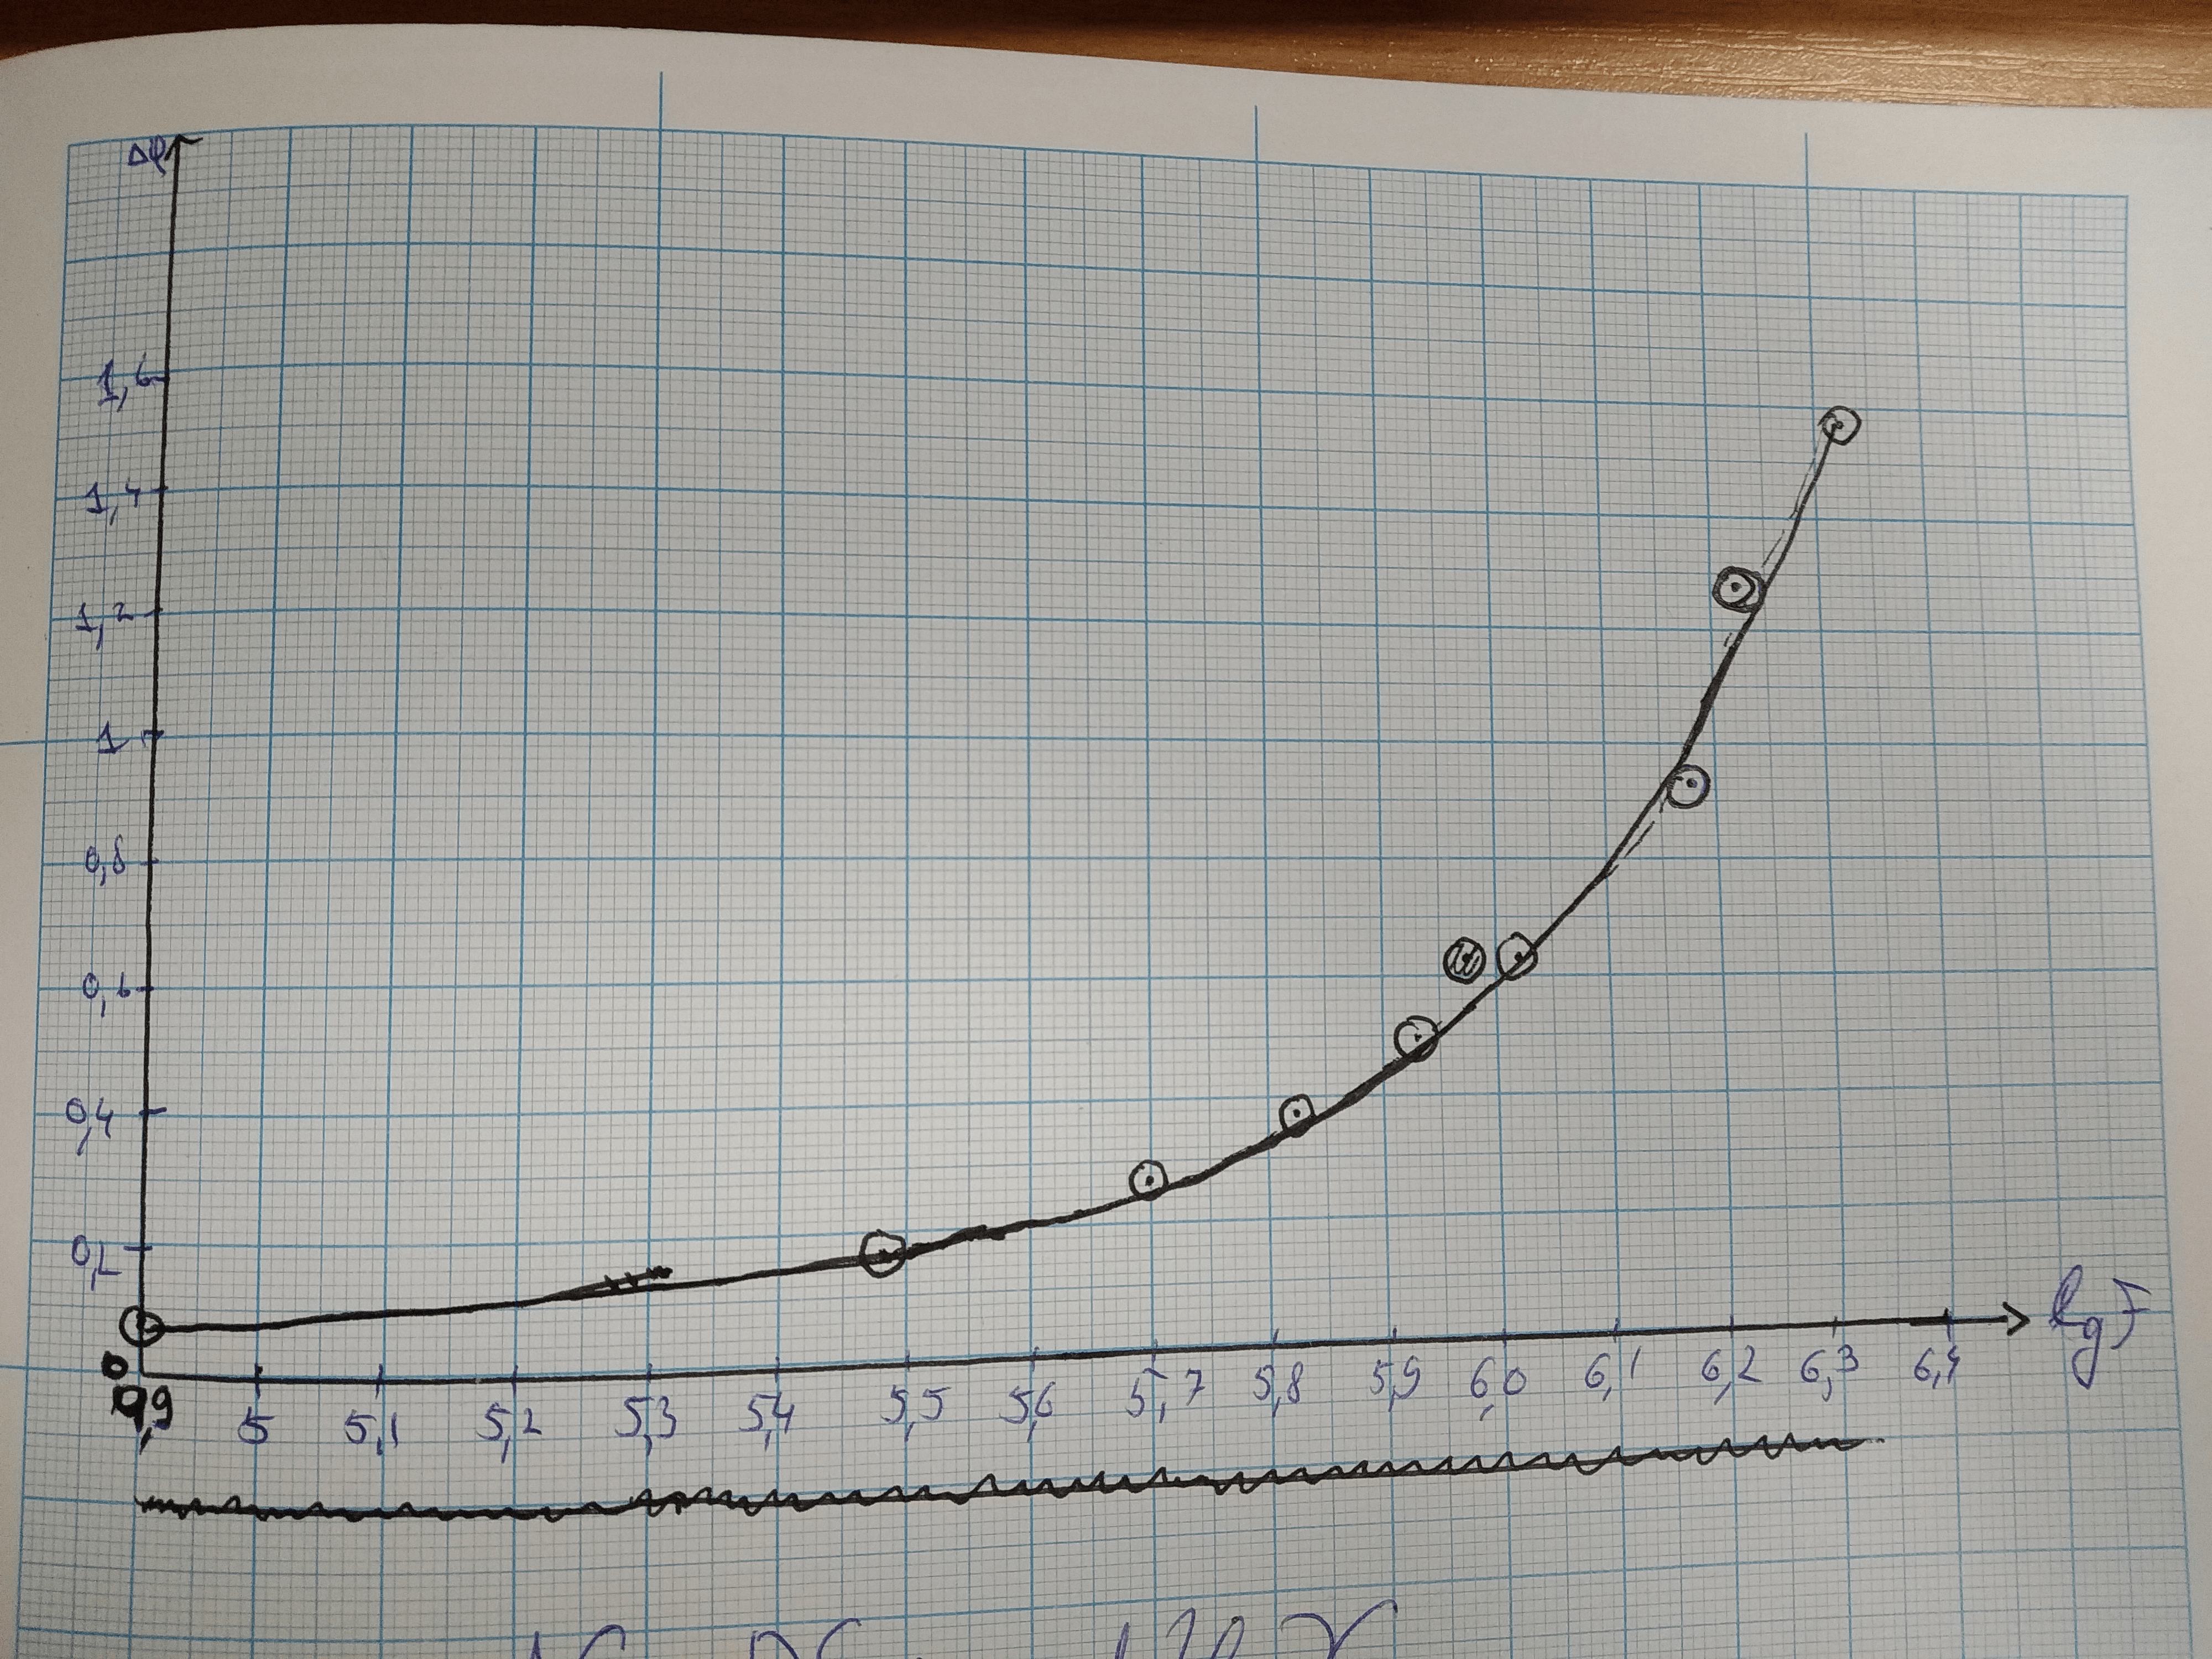
\includegraphics[width=120mm] 	{23}
\end{center}

\begin{center}
\includegraphics{24}
\end{center}

\begin{center}
\includegraphics{25}
\end{center}

\begin{center}
\includegraphics{26}
\end{center}






\end{document}


